\newpage
\subsection{Tratamiento de datos ausentes}
En este parte del análisis exploratorio de datos oncológicos, se detectaron, imputaron y posteriormente se eliminaron las variables innecesarias identificadas en el análisis parcial de datos genómicos crudos, por medio de algoritmos en \textit{Python}.

\subsubsection{Detección de datos ausentes}
En esta parte del tratamiento de datos ausentes, se identificaron si las \textit{69 variables} identificadas anteriormente seguían presentando inconsistencias o datos faltantes. Dado lo anterior, se realizo nuevamente un análisis de la cantidad de \textbf{datos ausentes} pero esto vez a través del \textit{mapa espectral} que se observa en la figura \ref{Missing_Spectrum}. Este tipo de gráfico se utilizó debido a que permite visualizar la trama de datos que faltan en un registro determinado, por lo cual fue posible conocer que datos debían ser imputados.

\subsubsection{Imputación de datos ausentes}
En esta parte del tratamiento de datos ausentes, se completaron los datos faltantes haciendo uso de la librería  \textit{sklearn.impute} la cual proporciona algoritmos de ML para la imputación de datos. 
 
Dado lo anterior, en este caso se utilizó la función \textit{impute.KNNImputer()} para tratar los datos de tipo \textit{numérico}. Este modelo detecta los valores faltantes de cada muestra y los imputa utilizando el valor medio de vecinos más cercanos que se encuentran en el conjunto de entrenamiento. En el algoritmo \ref{imputacion_num} se puede observar el código implementado.
 
 \begin{lstlisting}[basicstyle=\scriptsize,language=Python, label=imputacion_num, caption=Imputar datos numéricos con sklearn en Python.]
 	from sklearn.impute import KNNImputer
 	
 	# Imputar variables numericas
 	imputer = KNNImputer(n_neighbors=5, weights="distance")
	imput_data=['diagnosis_age', 'cent_17_copy_number', 'birth_initial_diagnosis', 'days_sample_collection', 'her_2_cent_17_ratio', 'disease_free_months', 'days_last_followup', 'year_initial_diagnosis', 'positive_lymph_hematoxylin', 'lymph_examined_number', 'mutation_count', 'overall_survival_months', 'tmb_nonsynonymous' ]
 	
 	for i in imput_data :
 	bc[i]=bc[i].replace([0.0,0,'0','0.0'],[np.nan,np.nan,np.nan,np.nan])
 	
 	# Ajustamos el modelo e imputamos los datos numericos
 	imputer.fit(bc[[i]])
 	bc[i] = imputer.transform(bc[[i]]).ravel()
 	bc[i] = round(bc[i],1)
 \end{lstlisting}
 
 Así mismo, se utilizó la función \textit{impute.SimpleImputer()} para tratar los datos de tipo \textit{categórico}. Este modelo reemplaza los valores faltantes usando una estadística descriptiva (p. ej., media, mediana o más frecuente) a lo largo de cada columna, o usando un valor constante. En el algoritmo \ref{imputacion_cat} se puede observar el código implementado.
  
   \begin{lstlisting}[basicstyle=\scriptsize,language=Python, label=imputacion_cat, caption=Imputar datos categóricos con sklearn en Python.]
  	from sklearn.impute import SimpleImputer
  	
	# Imputar variables categoricas
	mode_data=['neoplasm_disease_stage_code',
	'brachytherapy',
	'publication_version_type',
	'er_positivity_scale_used',
	'cancer_type_detailed',
	'disease_free_status',
	'er_positivity_scale_other',
	'er_status_ihc_percent_positive',
	'ethnicity_category',
	'surgical_other',
	'er_status_ihc',
	'her_2_fish_status',
	'her_2_ihc_score',
	'her_2_ihc_percent_positive',
	'neoplasm_histologic_type',
	'neoadjuvant_therapy',
	'prior_diagnosis_occurence','ihc_her_2','ihc_score',
	'lymph_presentation',
	'menopause_status',
	'metastatic_tumor_indicator',
	'biospecimen_method',
	'micromet_detection_ihc',
	'oct_embedded',
	'disease_surgical_margin_status',
	'primary_tumor_site',
	'tissue_prospective_indicator',
	'pr_positivity_define_method',
	'pr_positivity_scale_other',
	'positive_lymph_keratin',
	'pr_status_ihc',
	'pr_status_ihc_percent_positive',
	'pr_positivity_ihc_intensity_score',
	'pr_positivity_scale_used',
	'race_category','tissue_retrospective_indicator',
	'staging_system',
	'surgical_procedure_first',
	'tissue_source_site','person_neoplasm_status'
	]
  		
  	# Ajustamos el modelo e imputamos los datos categoricos
  	for i in mode_data :
	  	bc[i]=bc[i].replace([0.0,0,'0','0.0'],[np.nan,np.nan,np.nan,np.nan])
	  	bc[i] = bc[i].fillna(bc[i].mode()[0])
	  	imputer = SimpleImputer(strategy='most_frequent', 
	  	missing_values=np.nan)
	  	imputer = imputer.fit(bc[[i]])
	  	bc[[i]] = imputer.transform(bc[[i]])
  \end{lstlisting}
 
 
\subsubsection{Eliminación de datos ausentes}

En esta parte del tratamiento de datos ausentes, se eliminaron \textit{69 variables}, ya que una vez realizada la imputación de datos, se confirmo que efectivamente no brindaban informacion relevante para responder las preguntas planteadas en el \textit{BCQM}, la cantidad de datos no ERA suficiente para generar un análisis verídico o  no aportaban información de índole genético relacionada con los tipos de cáncer Lobulillar Invasivo (LBC), Ductal Invasivo (IDC) o de Tumores Mixtos (MTBC). En el algoritmo \ref{eliminacion} se puede observar el código implementado.
 
  \begin{lstlisting}[basicstyle=\tiny,language=Python, label=eliminacion, caption=Eliminar datos poco relvantes en Python.]
	#Eliminar variables inncesarias
	bc=bc.drop(
	[
	'study_id',
	'patient_id',
	'sample_id',
	'cancer_type',
	'death_initial_diagnosis',
	'last_alive_date',
	'publication_version_type',
	'disease_code',
	'brachytherapy',
	'form_completion_date',
	'histology_code',
	'site_code',
	'cent_17_copy_number',
	'birth_initial_diagnosis',
	'pr_positivity_define_method',
	'er_positivity_scale_used',
	'er_positivity_scale_other',
	'her_2_cent_17_cells_count',
	'her_2_cent_17_scale_other',
	'her_2_copy_number',
	'her_2_cent_17_ratio',
	'her_2_fish_method',
	'her_2_positivity_method_text',
	'her_2_positivity_scale_other',
	'tumor_other_subtype',
	'consent_verified',
	'is_ffpe',
	'ihc_score',
	'margin_status_reexcision',
	'prior_diagnosis_occurence',
	'metastatic_site',
	'metastatic_site_other',
	'biospecimen_other_method',
	'new_neoplasm_event',
	'icd_10_classification',
	'nte_cent_17_her_2_ratio',
	'nte_er_ihc_intensity_score',
	'nte_er_status',
	'nte_er_status_ihc_positive',
	'nte_her_2_fish_status',
	'nte_her_2_positivity_ihc_score',
	'nte_her_2_status',
	'nte_her_2_status_ihc_positive',
	'nte_pr_ihc_intensity_score',
	'nte_pr_status_ihc','nte_pr_status_ihc_positive',
	'other_patient_id','other_sample_id',
	'pathology_report_file_name','pharmaceutical_therapy',
	'project_code','positive_lymph_keratin',
	'tissue_retrospective_indicator','pr_positivity_ihc_intensity_score',
	'pr_status_ihc_percent_positive','pr_positivity_scale_other',
	'pr_positivity_scale_used','postoperative_radiotherapy',
	'number_samples','sample_type',
	'somatic_status','staging_system_1',
	'surgery_positive','surgery_positive_other','surgical_other',
	'tissue_source_site','tumor_disease_anatomic_site',
	'days_sample_collection','days_last_followup'
	], axis=1)
 \end{lstlisting}

\subsubsection{Consistencia de datos}
En esta parte del tratamiento de datos ausentes, se comprobó que las variables que se quedaran correctamente imputadas y si ningún dato incompleto. Dado lo anterior, los resultados obtenidos de la estandarización de los datos se pueden observar en el \textit{mapa espectral} que se observa en la figura \ref{impute_Spectrum}. Para una mayor trazabilidad en la tabla \ref{data_limpia} se observan las 41 variables que fueron seleccionadas para realizar el análisis descriptivo de datos.
\begin{figure}[htb!]
	\centering
	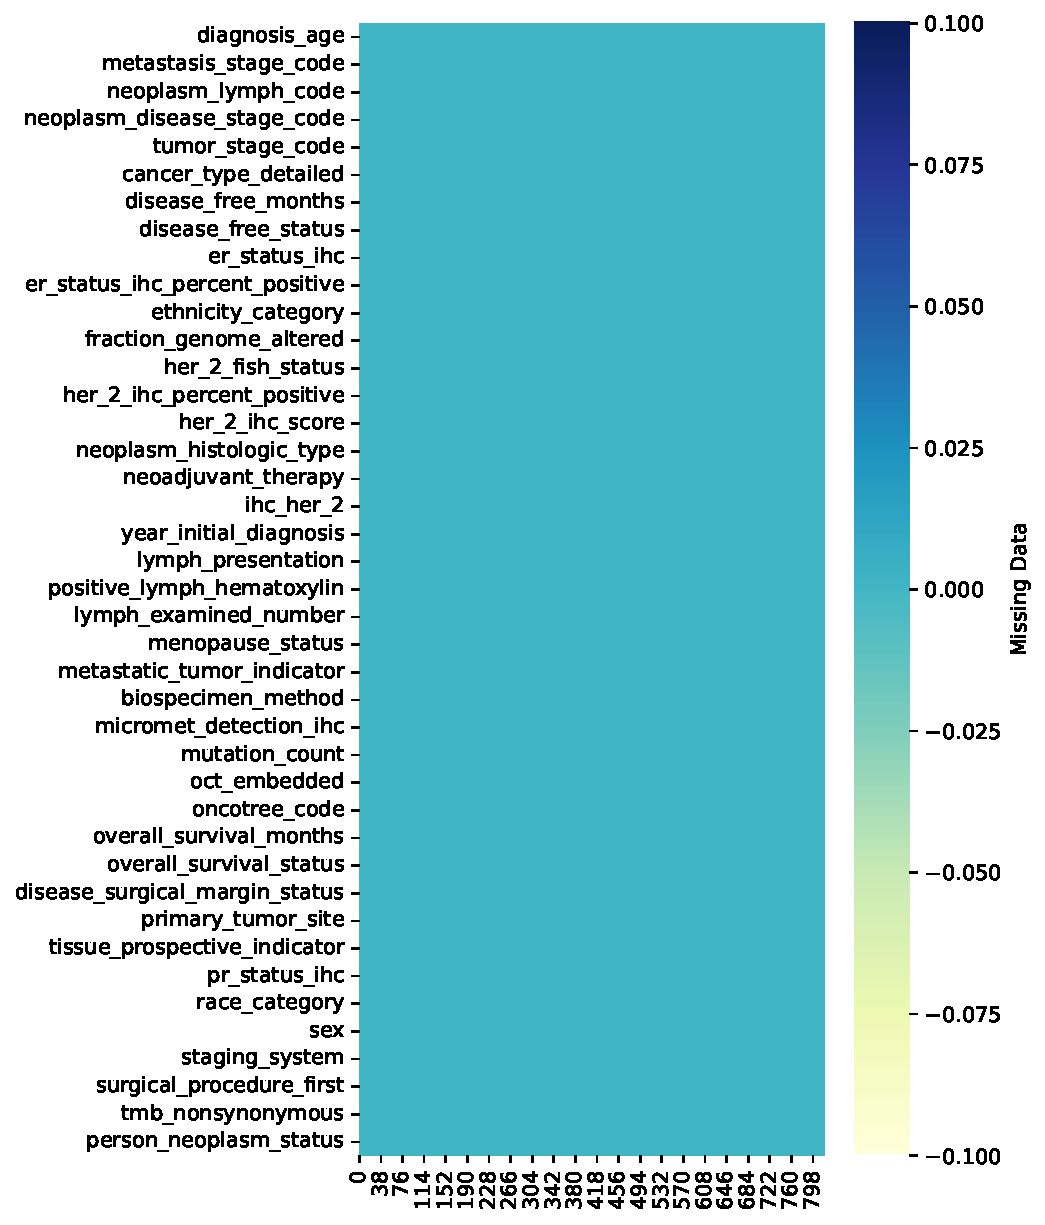
\includegraphics[width=0.85
	\linewidth]{NOTEBOOK/IMAGENES_PERDIDAS/impute_heatmap}
	\caption{Datos imputados expresados en un mapa espectral.}
	\label{impute_Spectrum}
\end{figure}


\begin{table*}[hbt!]
	\footnotesize
	\centering
	\begin{threeparttable}
		\caption{Estadísticas de variables procesadas para el análisis descriptivo.}
		\label{data_limpia}
		\begin{tabular}{p{0.5cm} p{4cm} p{1.5cm} p{2cm} p{1.5cm} p{2cm} p{1.5cm}} \toprule
			$N$  &Variable &Distintas &Distintas($\%$) &Ausentes &Ausentes($\%$)  &Tamaño($kb$)
			\\ \hline	1	&	Diagnosis Age	&	65	&	7,9	&	0	&	0	&	12,8
			\\ \hline	2	&	Metastasis Stage Code	&	4	&	0,5	&	0	&	0	&	53,5
			\\ \hline	3	&	Neoplasm Disease Lymph Node Stage AJCC Code	&	16	&	2	&	0	&	0	&	54,5
			\\ \hline	4	&	Neoplasm Disease Stage AJCC Code	&	12	&	1,65	&	0	&	0	&	59
			\\ \hline	5	&	AJCC Tumor Stage Code	&	12	&	1,5	&	0	&	0	&	53,7
			\\ \hline	6	&	Cancer Type Detailed	&	4	&	0,5	&	0	&	0	&	77,6
			\\ \hline	7	&	Disease Free 	&	458	&	56	&	0	&	0	&	12,8
			\\ \hline	8	&	Disease Free Status	&	2	&	0,2	&	0	&	0	&	60,6
			\\ \hline	9	&	ER Status By IHC	&	2	&	0,2	&	0	&	0	&	58,3
			\\ \hline	10	&	ER Status IHC Percent Positive	&	10	&	1,2	&	0	&	0	&	56,6
			\\ \hline	11	&	Ethnicity Category	&	2	&	0,2	&	0	&	0	&	69,4
			\\ \hline	12	&	Fraction Genome Altered	&	754	&	92,2	&	0	&	0	&	12,8
			\\ \hline	13	&	HER2 fish status	&	2	&	0,2	&	0	&	0	&	58,3
			\\ \hline	14	&	HER2 ihc percent positive	&	10	&	1,2	&	0	&	0	&	55,2
			\\ \hline	15	&	HER2 ihc score	&	3	&	0,4	&	0	&	0	&	54,3
			\\ \hline	16	&	Neoplasm Histologic Type Name	&	8	&	1	&	0	&	0	&	74,1
			\\ \hline	17	&	Neoadjuvant Therapy 	&	2	&	0,2	&	0	&	0	&	53,5
			\\ \hline	18	&	IHC-HER2	&	4	&	0,5	&	0	&	0	&	58,5
			\\ \hline	19	&	Year Cancer Initial Diagnosis	&	27	&	3,2	&	0	&	0	&	12,8
			\\ \hline	20	&	Primary Lymph Node Presentation 	&	2	&	0,2	&	0	&	0	&	54,3
			\\ \hline	21	&	Positive hematoxylin Count	&	27	&	3,3	&	0	&	0	&	12,8
			\\ \hline	22	&	Lymph Node(s) Examined Number	&	42	&	5,1	&	0	&	0	&	12,8
			\\ \hline	23	&	Menopause Status	&	3	&	0,4	&	0	&	0	&	55
			\\ \hline	24	&	Metastatic tumor indicator	&	2	&	0,2	&	0	&	0	&	53,5
			\\ \hline	25	&	First Pathologic Diagnosis 	&	7	&	0,9	&	0	&	0	&	65,9
			\\ \hline	26	&	Micromet detection by ihc	&	2	&	0,2	&	0	&	0	&	53,7
			\\ \hline	27	&	Mutation Count	&	165	&	20,2	&	0	&	0	&	12,8
			\\ \hline	28	&	Oct embedded	&	2	&	0,2	&	0	&	0	&	55,4
			\\ \hline	29	&	Oncotree Code	&	4	&	0,5	&	0	&	0	&	54,5
			\\ \hline	30	&	Overall Survival	&	506	&	61,9	&	0	&	0	&	12,8
			\\ \hline	31	&	Overall Survival Status	&	2	&	0,2	&	0	&	0	&	57
			\\ \hline	32	&	Disease Surgical Margin Status	&	3	&	0,4	&	0	&	0	&	58,2
			\\ \hline	33	&	Primary Tumor Site	&	10	&	1,2	&	0	&	0	&	57,5
			\\ \hline	34	&	Tissue Prospective 	&	2	&	0,2	&	0	&	0	&	61,8
			\\ \hline   35	&	PR status by ihc	&	2	&	0,2	&	0	&	0	&	58,3
			\\ \hline	36	&	Race Category	&	4	&	0,5	&	0	&	0	&	57,7
			\\ \hline	37	&	Sex	&	2	&	0,2	&	0	&	0	&	56,7
			\\ \hline	38	&	Staging System	&	5	&	0,6	&	0	&	0	&	80,3
			\\ \hline	39	&	Surgical procedure first	&	4	&	0,5	&	0	&	0	&	64,1
			\\ \hline	40	&	TMB (nonsynonymous)	&	83	&	10,2	&	0	&	0	&	12,8
			\\ \hline	41	&	Person Neoplasm Status	&	2	&	0,2	&	0	&	0	&	59,9
			\\ \hline
		\end{tabular}
	\end{threeparttable}
\end{table*}

\clearpage